
\section{Introduction}

While it is a common understanding in the field that deeper networks are better\cite{ba2014deep}; in practice training a very deep network for the same size data is prone to over-fitting and vanishing gradients. Recently, some success has been observed by techniques which minimize the attenuation of the information by either learning to represent the residues\cite{he2015deep} or by adding gating units which reinforce the original signal\cite{srivastava2015highway}. This allows successful training of network with thousands of layers.

For the task of visual question answering, we propose a network which alters the gating units to be feed by multi dimensional representation of the words from the question. This allows us to learn common feature space in a single end to end training. When the length of question is shorter than the number of layers, it can be either padded with zeros or by repeating the words from the question. We present our model and result from the VQA dataset\cite{antol2015vqa}. 

\begin{figure}[H]
\centering
   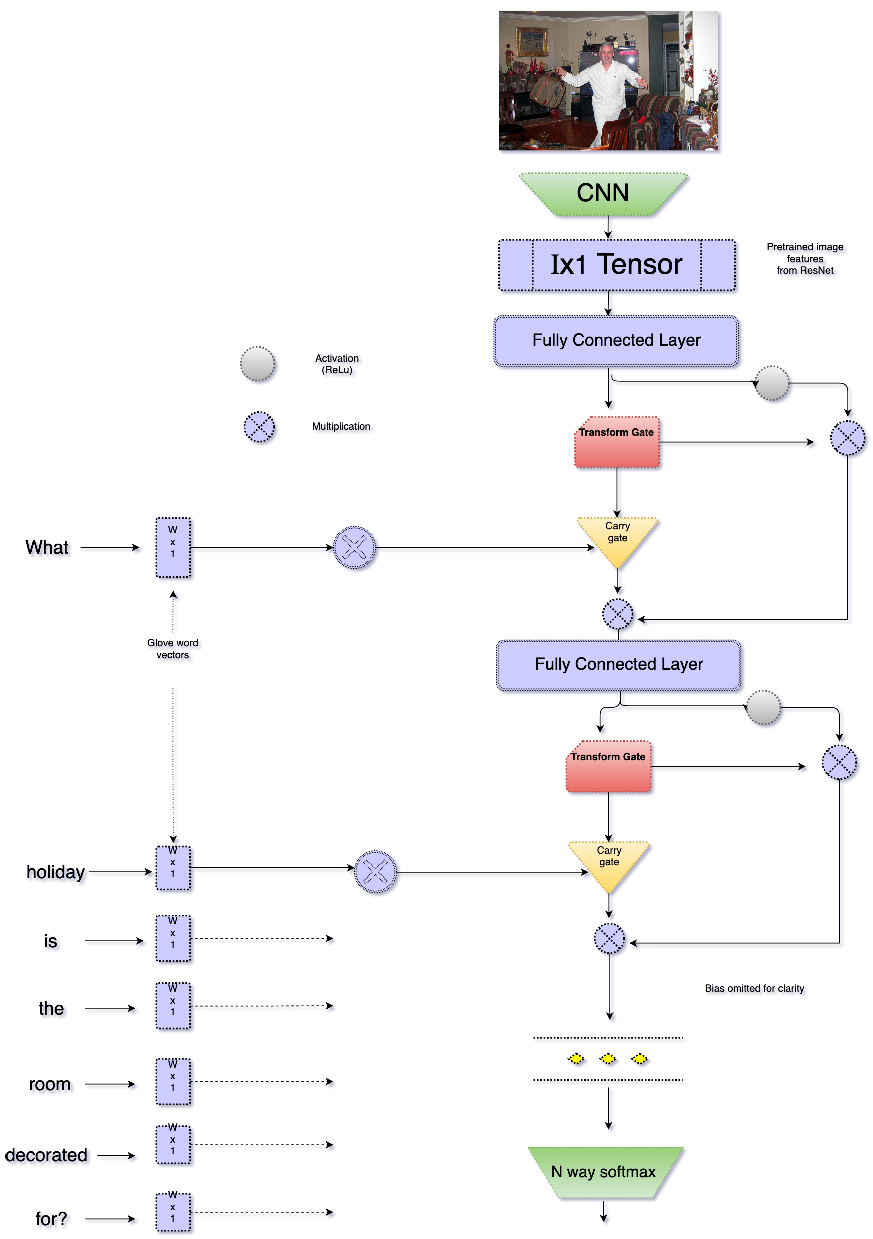
\includegraphics[width=1\linewidth, scale=0.9]{figures/vqa/model.pdf}
    \caption{Architecture of multi-modal highway networks}
    \label{fig:long}
    \label{fig:onecol}
\end{figure}
%-------------------------------------------------------------------------
\subsection{Highway Networks}

For the given input $x$, and weight matrix $\boldmath{W}$, a feed forward network tries to learn the following representation --
\begin{displaymath}
y = H(x, \boldmath{W}) + \mathbf{b}
\end{displaymath}
where, $H$ is a non-linear transformation and $\mathbf{b}$ is bias. Highway Network as described by Srivastava et al\cite{srivastava2015highway}, adds two gates to above equation, essentially transforming it to --
\begin{displaymath}
y = H(x, \boldmath{W_H})\cdot T(x, \boldmath{W_T}) + x \cdot C(x,\boldmath{W_C})
\end{displaymath}



where, T and C are \textit{transform} gate and \textit{carry} gate.  It should be noted that \boldmath{x}, \boldmath{y}, \boldmath{H}, \boldmath{T}, and \boldmath{C} should have same dimensionality.

\subsection{Gating for Visual Question Answering}
Since the original model was meant for a single learning task like image classification, the authors choose the carry gate $\boldmath{C} = \boldmath{1-T}$, the same cannot be done for multimodal learning like visual question answering. 

Our modification for the carry gate is to feed the word vectors of the words from the question, extracted from pre-trained models like Glove vectors\cite{pennington2014glove} . $K\times1$ features from word embeddings are translated to dimensions of '$x$' by point-wise multiplication. At each layer vector from only one word or average of few words are feed. This allows us to learn temporal relationship in the words in question. However, for this task, individual words in any order seem to perform equally well. 

%-------------------------------------------------------------------------
\subsection{Feature space}

Most of the related work on visual question answering use some form of pre-trained image vector. All the models used are trained on ImageNet images, and the last layer before the softmax is extracted. It is common to use GoogLeNet \cite{jiang2015compositional} \cite{xu2015ask} \cite{zhou2015simple} \cite{wu2016image} or VGGNet \cite{wu2015ask}  \cite{xiong2016dynamic}  \cite{yang2015stacked}   \cite{shih2015look} \cite{ren2015exploring} \cite{andreas2016learning} \cite{Lu2015}\cite{zhu2015visual7w} \cite{noh2015image}. We use ResNet\cite{he2015deep} for their ability to extract better features. Features obtained from VGGNet, GoogLeNet or ResNet are easily transferable to MS COCO Images and  number of images in the VQA dataset are not big enough to train a independent image model. However, some of the models do fine-tuning\cite{noh2015image}, but with our model that is redundant because the \textit{transfer gate} alters the weights of image features effectively doing fine-tuning constrained upon {carry gate} weights.

%-------------------------------------------------------------------------
\subsection{Attention}
Most of the recent models \cite{xiong2016dynamic} \cite{xu2015ask} \cite{yang2015stacked} tackling the task of visual question answering have taken inspiration from success of soft attention models for image captioning\cite{karpathy2015deep} \cite{xu2015show}. This has led to some improvement in VQA but comes at a cost of slower training process due to recurrent network. While Noh et. al's \cite{noh2015image} use of parameter prediction to obtain attention from hashing weights into smaller dimension and Xiong et. al's\cite{xiong2016dynamic} use of episodic memory for attention avoids recurrence but are limited by size of learnable parameters. Our model achieves the effect of attention by learning the parameters of the gate. And thus it can be extended by adding more layers. \textit{Carry gate} changes the network structure based on the improvement obtained from merging the weights from current word vector.  In a control experiment where question words were replaced by random words, the network performance was diminished significantly.

\subsection{Bi-directional Recurrence}
As an experimental model we appended with input questions in reverse order. This improved the accuracy of the model only slightly but the computational cost was doubled and training took twice the time. Thus we believe there is not much gain in bi-directional recurrence as far as visual question answering is concerned. Similar results were reported for bi-directional LSTM by Ren et al \cite{ren2015exploring}.

%-------------------------------------------------------------------------
\section{Results}

\begin{table}[H]
\centering
\rowcolors{1}{White}{Gray}
\caption{Results of VQAv1}
\label{my-label}
\begin{tabular}{|l|l|l|l|l|l| l|}
\hline
%\multicolumn{1}{|c|}{} 
  & \multicolumn{5}{|c|}{Open Ended}  & MC  \\
  \hline
 & \multicolumn{4}{|c|}{Test-Dev}  & \multicolumn{2}{|c|}{Test-Std} \\
\hline


\textbf{Method} & \textbf{All}  &\textbf{ Y/N}  & \textbf{Other}  & \textbf{Num} & \textbf{All} & \textbf{All}  \\ \hline \hline
Image only& 28.1& 64.0& 3.8& 0.4& - & 30.5\\ \hline
Question only& 48.1& 75.7& 27.1& 36.7& - & 53.6\\ \hline
Q+I& 52.6& 75.6& 37.4& 33.7& - & 58.9\\ \hline
LSTM Q+I& 53.7& 78.9& 36.4& 35.2& 54.1 & 57.1\\ \hline
CMV \cite{jiang2015compositional} & 52.6& 78.3& 35.9& 34.4& - & -\\ \hline 
AMA \cite{wu2015ask} & 55.7& 79.2& 40.1& 36.1& 56.0 & -\\ \hline
iBOW \cite{zhou2015simple} & 55.7& 76.5& 42.6& 35.0& 55.9 & 61.9\\ \hline
DPPNet \cite{noh2015image}& 57.2& 80.7& 41.7& 37.2& 57.4 & 62.6\\ \hline
LCN \cite{andreas2016learning} & 57.9& 80.5& 43.1& 37.4& 58.0 & -\\ \hline
AAA \cite{xu2015ask} & 57.9& 80.8& 43.2& 37.3& 58.2 & -\\ \hline
dLSTM+ \cite{Lu2015} & 57.7& 80.5& 43.0& 36.7& 58.1 & 63.0\\ \hline
SAN \cite{yang2015stacked} & 58.7& 79.3& 46.1& 36.6& 58.9 & -\\ \hline
DMN+ \cite{xiong2016dynamic} & 60.3& 80.5& 48.3& 36.8& 60.4 & -\\ \hline
\textbf{OUR} & \textbf{60.4}& \textbf{81.5}& \textbf{47.6}& \textbf{37.2}& \textbf{60.7} & \textbf{65.0} \\ \hline

\end{tabular}
\end{table}
